\begin{surferPage}[הֶפטַגוֹן]{A משטח הפטגונלי סימטרי}
    זהו משטח ממעלה $7$ הנראה כמו כוכב.  
    עד לאחרונה, מספר נקודות הסינגולריות שלו, $84$, נחשב עדיין
    למספר המרבי של נקודות סינגולריות ממשיות במשטחים ממעלה שבע;
    רק בשנת 2004, שבר אוליבר לאבס (Oliver Labs) את השיא הזה עם משטח בעל $99$ נקודות סינגולריות.
  
  
 שלוש הכריות הנראות בתצוגה האינטראקטיבית, 
    נוצרות כתוצאה מהשימוש בפולינומים של צֶ'בּישֶב (Chebychev), הדומים לפולינום צ'מוטוב (Chmutov) מהמעלה השמינית.
    . 
    למעשה, המשטח דמוי-הכוכב הוא גרסה שונה של משטחי צ'מוטוב.
    במקרה זה, עקומת המישור $T_d(x)+T_d(y)$ הוחלפה על-ידי הפטגון משוכלל
    $S_7(x,y)$: 
   \[S_7(x,y) + \lambda \cdot T_d(z) = 0,\]
    עבור $\lambda\in\RR$. 
    \vspace*{-0.3em}
    \begin{center}
      \begin{tabular}{c@{\qquad}c}
        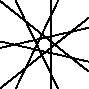
\includegraphics[height=1.5cm]{./../../common/images/labsseptic1.pdf}
        &
        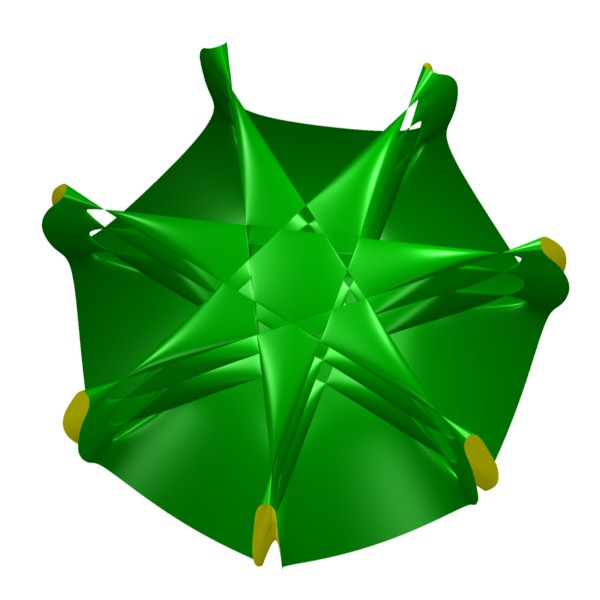
\includegraphics[height=1.5cm]{./../../common/images/septic_7eck_von_oben}
      \end{tabular}
    \end{center}
    \vspace*{-0.3em}   
   גרסה זו של מבנה צ'מוטוב היא באדיבות דוקו ואן-סטראטן (Duco van Straten).
\end{surferPage}
